\subsection{Schwerpunkt Physik der Informationstechnologie}
\label{subsec:studienstruktur_schwerpunkt_it_bsc}
Bei der \fach{Physik der Informationstechnologie} handelt es sich um einen Schwerpunkt, den ihr im Laufe eures Physikstudiums erwerben könnt. Hierfür wird auf die Wahlfreiheit des Nebenfachs und der Wahlpflicht-Fächer zugunsten einer Spezialisierung in der Informationstechnologie verzichtet. Ihr erhaltet einen tieferen Einblick in die Grundlagen der Programmierung und lernt die physikalischen Konzepte der Informationstechnologie. Auf den Informatikanteil der Ausbildung wird also ein grö\ss eres Augenmerk als beim regulären Physikstudium gelegt.\\
Die ersten drei Semester unterscheiden sich nicht vom Physikstudiengang ohne Schwerpunkt. Die Entscheidung für den Schwerpunkt sollte mit Beginn des vierten Semesters getroffen werden, damit ihr im regulären Studienablauf bleibt und ihr das für Physiker verpflichtende Programmierpraktikum mit den Informatikvorlesungen ersetzten könnt.\\
Habt ihr euch für den Schwerpunkt entschieden, beginnt ihr eure Spezialisierung, indem ihr zusätzlich zu den Physikvorlesungen des vierten Semesters die Veranstaltungen \VL{Programmieren 2} für 8 CP und \VL{Datenstrukturen} für 5CP hört. Beide Vorlesungen finden in Bockenheim statt. Keine Sorge, \VL{Programmieren 1} kommt im nächsten Semester und beide Veranstaltungen können in beliebiger Reihenfolge gehört werden, da sie nicht auf einander aufbauen.\\
Von den Physikveranstaltungen im fünften Semester besucht ihr alle, au\ss er dem Programmierpraktikum. Dafür hört ihr jetzt die Vorlesung \VL{Programmieren 1} für 11 CP.\\
Neben den Physikveranstaltungen des 6. Semesters stehen noch die \VL{Halbleiter und Bauelemente}--Vorlesung für 4 CP und die unbenotete Vorlesung \VL{Hardwarearchitektur und Rechensysteme} für 8 CP auf dem Plan.\\
Alle Spezialvorlesungen in diesem Schwerpunkt ersetzen die Noten für den Wahlpflicht- und den Nebenfachbereich. Sie gehen genauso wie diese mit 31 CP in die Bachelornote ein. Die Gesamtnote f\"ur den Schwerpunkt setzt sich aus den Noten für \VL{Halbleiter und Bauelemente} und zwei weitere Noten deiner Wahl aus den obengenannten Veranstaltungen zusammen.\\
Der Studiengang wird wie ein gewöhnlicher Physikstudiengang behandelt. Für die Informatikvorlesungen gelten, wie bei gewöhnlichen Nebenfächern, die Regelungen des Fachbereichs Informatik. \\
Der Erwerb dieses Schwerpunktes wird im Bachelorzeugnis festgehalten und ermöglicht ein Studium des Masters \VL{Physik der Informationstechnologie}.
\newpage
\subsection{Master Physik mit Schwerpunkt Informationstechnologie}
\label{subsec:studienstruktur_schwerpunkt_it_msc}
Au\ss er dem normalen Physik-Master gibt es in Frankfurt auch den Physik-Master mit Schwerpunkt Informationstechnologie. Solltet ihr diesen wählen, müsst ihr das zu Beginn eures Masterstudiums erklären. Im Gegensatz zum reinen Physik-Master hat man hier kein frei wählbares nichtphysikalisches Nebenfach. Stattdessen müsst ihr 20--24 CP aus den Wahlpflichtmodulen Physik und 16--20 CP aus den Wahlpflichtmodulen Informatik erbringen, sodass ihr in der Summe auf 40 CP kommt. Dabei wird aus der Informatik das Modul \Modul{B-GL 1} empfohlen. Mögliche Themen für die Abschlussarbeit sind auf Gebiete der Physik der Informationstechnologie (z.B. Physik der Computerhardware) beschränkt. Im Zweifelsfall entscheidet der Prüfungsausschuss und es wird dringend empfohlen, dass Thema einer geplanten Abschlussarbeit vorher auf Zulässigkeit prüfen zu lassen. Die Pflichtmodule und die Prüfungsordnung sind die gleichen wie im reinen Physikmaster.
\begin{figure}
  \centering
  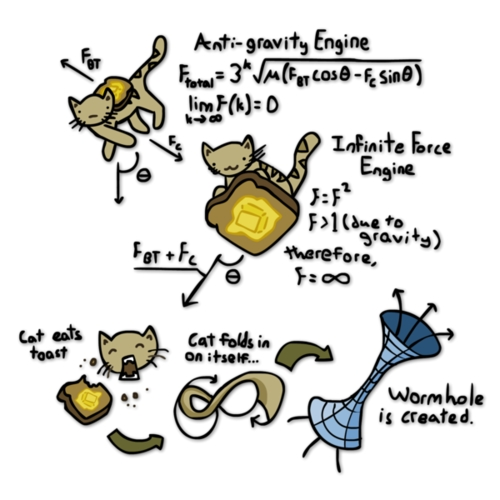
\includegraphics[height=.63\textheight]{\imgdir/Katze_Toast.jpg}
\end{figure}
\von{Daniela, Marco und Ole}